%% Преамбула TeX-файла

% 1. Стиль и язык
\documentclass[utf8x, 12pt]{G7-32} % Стиль (по умолчанию будет 14pt)


% Остальные стандартные настройки убраны в preamble.inc.tex.
\sloppy

% Настройки стиля ГОСТ 7-32
% Для начала определяем, хотим мы или нет, чтобы рисунки и таблицы нумеровались в пределах раздела, или нам нужна сквозная нумерация.
\EqInChapter % формулы будут нумероваться в пределах раздела
\TableInChapter % таблицы будут нумероваться в пределах раздела
\PicInChapter % рисунки будут нумероваться в пределах раздела

% Добавляем гипертекстовое оглавление в PDF
\usepackage[
bookmarks=true, colorlinks=true, unicode=true,
urlcolor=black,linkcolor=black, anchorcolor=black,
citecolor=black, menucolor=black, filecolor=black,
]{hyperref}
% Изменение начертания шрифта --- после чего выглядит таймсоподобно.
% apt-get install scalable-cyrfonts-tex

\IfFileExists{cyrtimes.sty}
    {
        \usepackage{cyrtimespatched}
    }
    {
        % А если Times нету, то будет CM...
    }

\usepackage{graphicx}   % Пакет для включения рисунков
\DeclareGraphicsExtensions{.jpg,.pdf,.png}
% С такими оно полями оно работает по-умолчанию:
\RequirePackage[left=30mm,right=15mm,top=20mm,bottom=20mm,headsep=0pt]{geometry}
\linespread{1.5}
% Если вас тошнит от поля в 10мм --- увеличивайте до 20-ти, ну и про переплёт не забывайте:
%\geometry{right=20mm}
%\geometry{left=30mm}



% Произвольная нумерация списков.
\usepackage{enumerate}
\usepackage{color, colortbl}
\definecolor{Red}{rgb}{0.8,0.2,0.1}
\definecolor{green}{rgb}{0.1,0.9,0.1}
\definecolor{gray}{gray}{0.9}
\setlength\arrayrulewidth{1pt}
\setcounter{tocdepth}{2} %Подробность оглавления
%4 это chapter, section, subsection, subsubsection и paragraph
%3 это chapter, section, subsection и subsubsection
%2 это chapter, section, и subsection
%1 это chapter и section
%0 это chapter.


\begin{document}

\frontmatter % выключает нумерацию ВСЕГО; здесь начинаются ненумерованные главы: реферат, введение, глоссарий, сокращения и прочее.
\begin{center} 

\large Московский Государственный Универстит имени М. В. Ломоносова\\[5.5cm] 

\huge Реферат \\[0.6cm] % название работы, затем отступ 0,6см
\large на тему:  <<Интегрированные среды разработки ПО>>\\[3.7cm]


\end{center} 

\begin{flushright}
Выполнил: студент гр. 420 \\
Немешаева Алиса \\
\end{flushright}


\vfill 

\begin{center} 
\large Москва 2020
\end{center} 

\thispagestyle{empty}


\thispagestyle{empty}
\setcounter{page}{0}
\tableofcontents
\clearpage


\Introduction

Галактики не расположены случайным образом в пространстве. Они формируют собой особые структуры, 
такие как скопления и сверхскопления галактик. Эти структуры в свою очередь формируют собой цепи, 
или так называемые "нити".\\

\begin{figure}
    \center{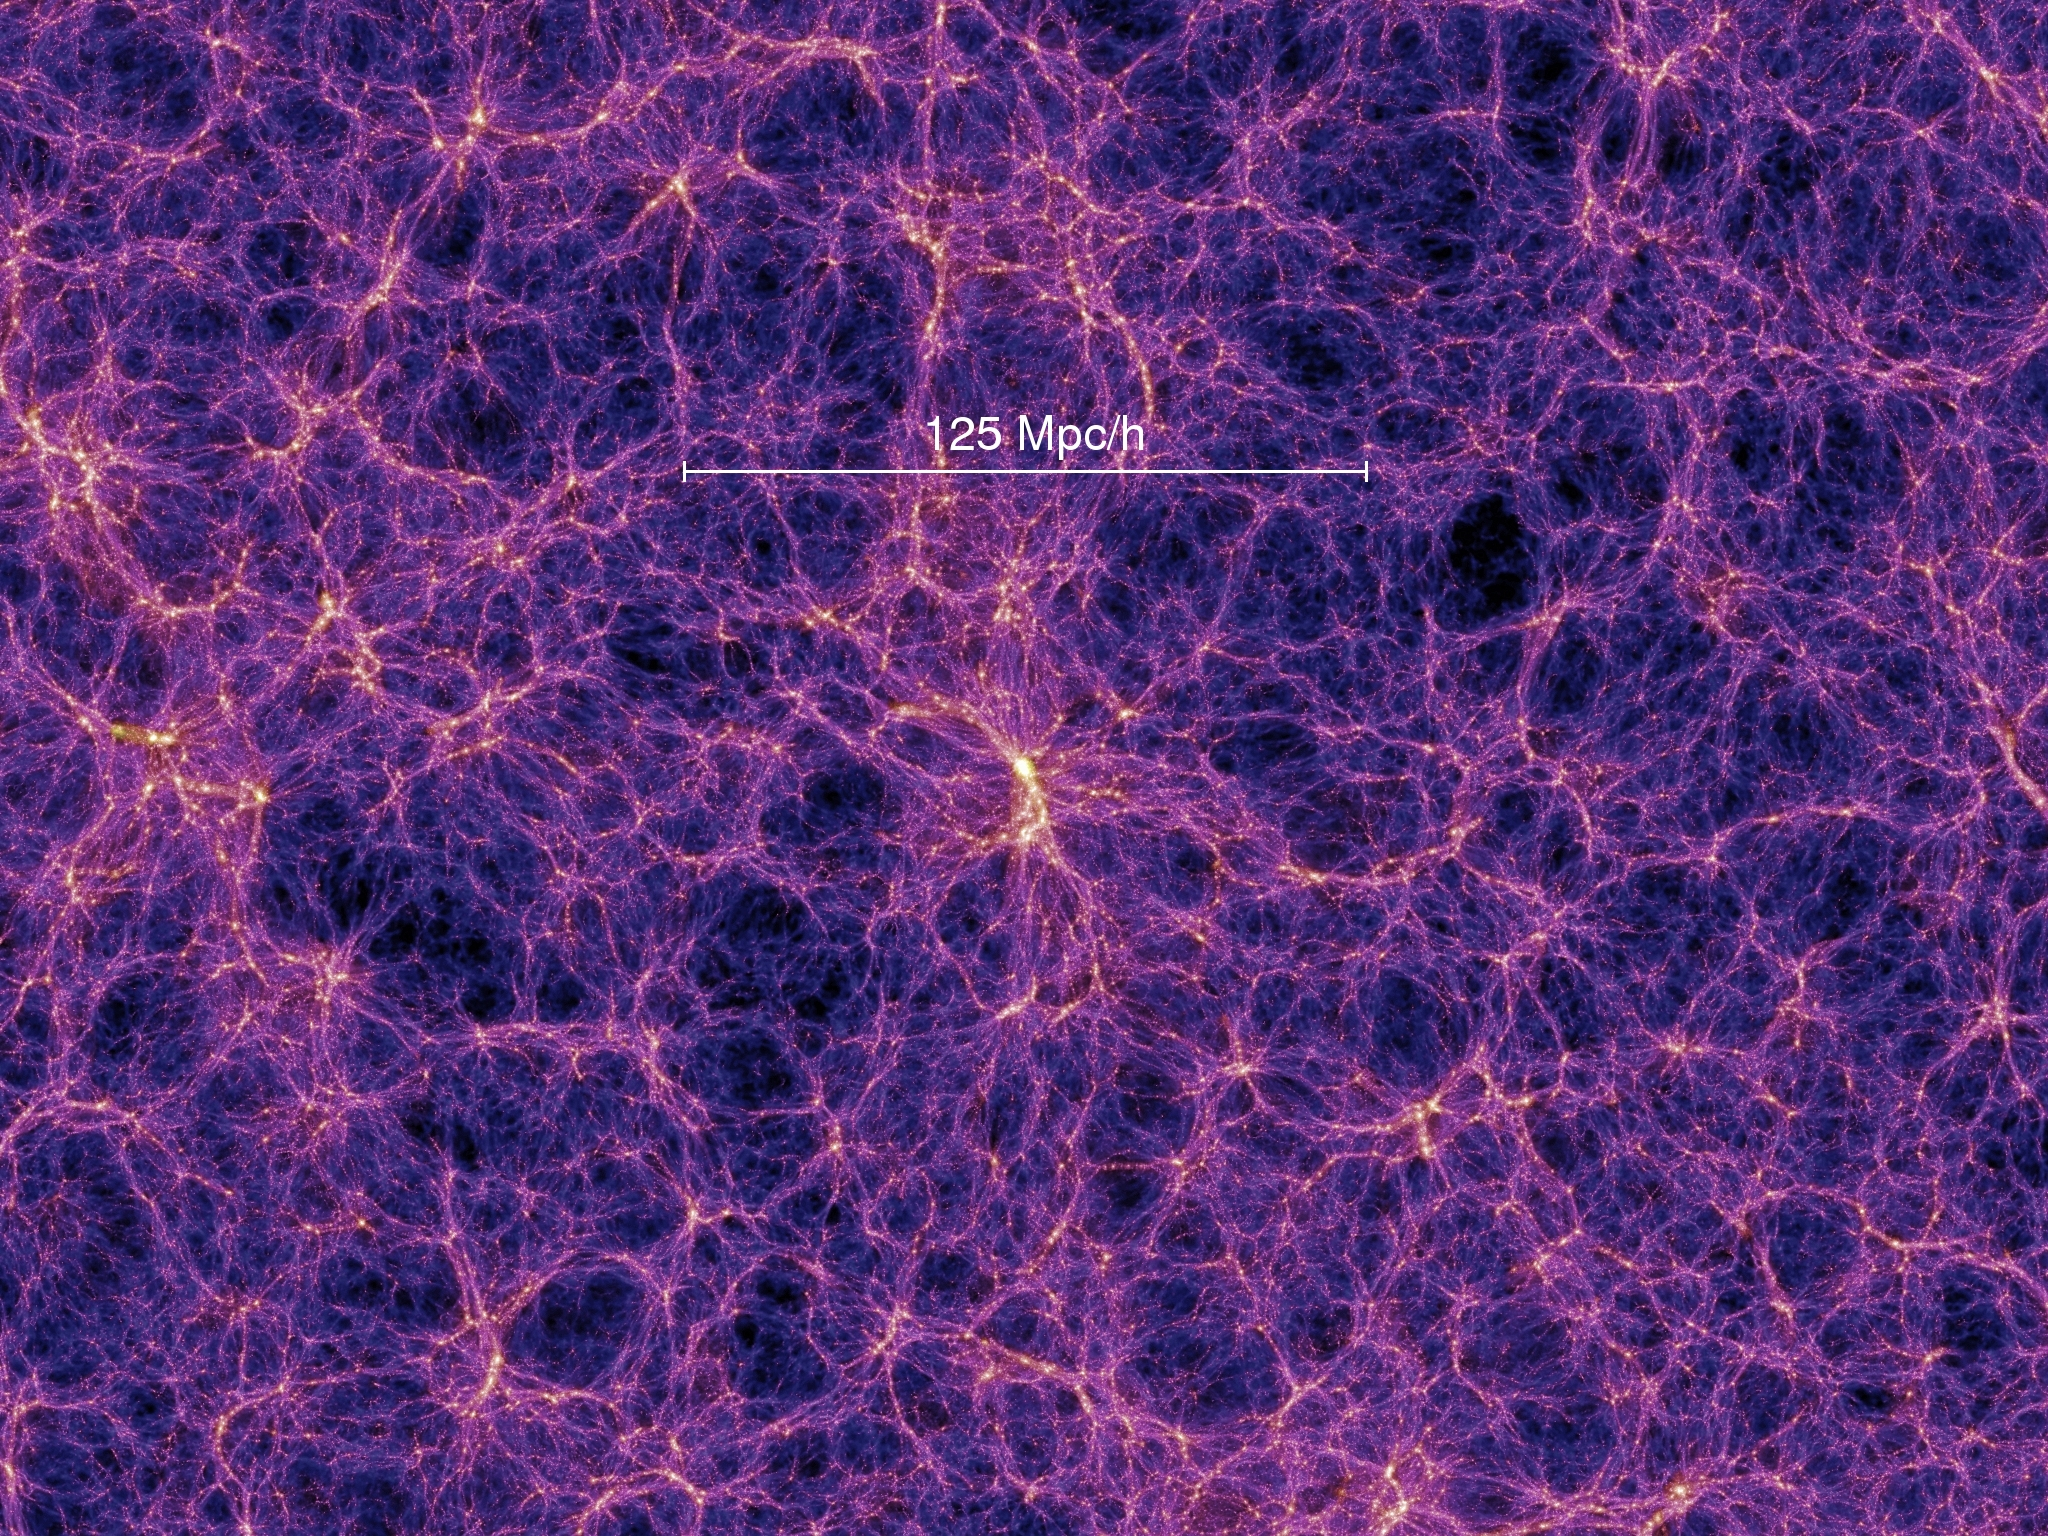
\includegraphics[width=0.6\linewidth]{model}}
    \caption{Моделирование «Милленниум» — N-частичное моделирование, проведённое Консорциумом 
        Девы с целью изучения формирования крупномасштабной структуры Вселенной в стандартной
        космологической модели.}
\end{figure}

Скопления галактик представляют большой интерес для исследования, так как их свойства сильно зависят 
от космологических параметров. Изучая их свойства, можно делать выводы о структуре обозримой части 
Вселенной.\\

Сама по себе крупномасштабная структура Вселенной имеет объяснение. При появлении Вселенной 
возмущения волн плотности средних и больших масштабов при совпадении пиков образовали сверхскопления,
в то время как сопадения фаз низкой плотности образовали войды - огромные пространства между нитями 
скоплений, в которых почти отсутствуют галактики и скопления. Таким образом, зная расположение и 
параметры большого количества скоплений, можно сделать выводы о том, как развивалась Вселенная на 
ранних этапах.\\

Одним из первых каталогов скоплений стал каталог Abell \cite{Abell}. Этот каталог содержит $4073$ 
богатых скопления галактик с красными смещениями $z < 0.2$. Он был построен при исользовании 
оптических данных обзора NGS-POSS.\\

\begin{figure}
    \center{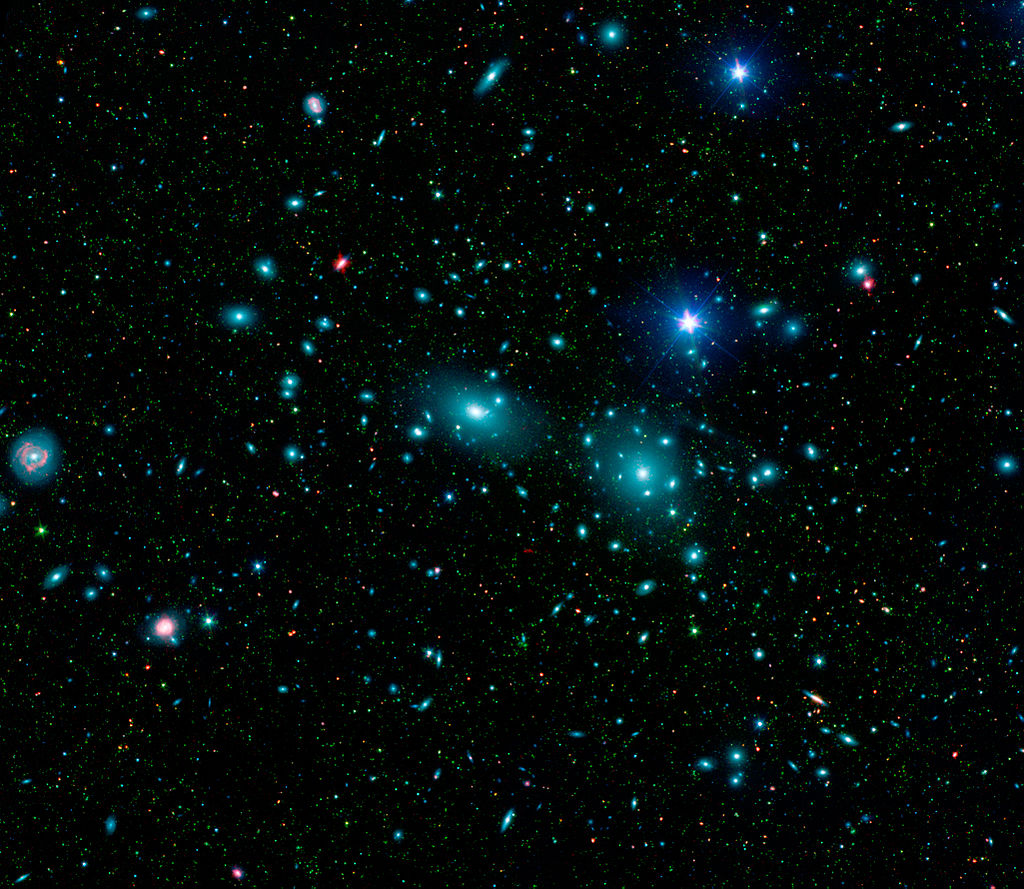
\includegraphics[width=0.6\linewidth]{coma_sdss}}
    \caption{Скопление Волос Вероники (Abell 1656) в обзоре SDSS - одно из самых известных 
        скоплений каталога Abell}
\end{figure}

Позднее были созданы каталоги с использованием других диапазонов. Далее для исследования будут 
использоваться следующие каталоги:\\

\section{PSZ2}

\section{MCXC}

\section{RedMaPPer}

\section{ACT}



\mainmatter

\chapter{История появления интегрированных сред разработки ПО}
\label{cha:ch_1}
Интегрированная среда разработки, ИСР (англ. IDE, Integrated Development Environment или Integrated Debugging Environment) — объединение программных средств, используемое разработчиками для создания программного обеспечения (ПО).\\
Классическая среда разработки включает в себя:\\
\begin{itemize}
    \item текстовый редактор;\\
    \item компилятор и / или интерпретатор;\\
    \item средства автоматизации сборки;\\
    \item отладчик.\\
\end{itemize}
Иногда IDE может содержать также средства для интеграции с системами управления версиями и различные инструменты для упрощения конструирования графического интерфейса для конечного пользователя. 
Современные среды разработки часто также включают браузер классов, инспектор объектов и диаграмму иерархии классов — для упрощения систематизации при объектно-ориентированной разработке ПО. 
Хотя и существуют IDE, предназначенные для нескольких языков программирования — такие, как Eclipse, NetBeans, Embarcadero RAD Studio, Qt Creator или Microsoft Visual Studio, но чаще всего IDE предназначается для одного определённого языка программирования - как, например, Visual Basic, PureBasic, Delphi, Dev-C++.\\

Первые IDE были созданы для работы через консоль или терминал, которые сами по себе только недавно вошли в употребление на тот момент времени: до того программы создавались на бумаге, вводились в машину с помощью предварительно подготовленных бумажных носителей (перфокарт, перфолент) и так далее.\\

Dartmouth BASIC был первым языком, который был создан с IDE, и был также первым языком, что был разработан для использования в консоли или терминале. Эта IDE (часть Dartmouth Time Sharing System) управлялась при помощи команд, поэтому существенно отличалась от более поздних, управляемых с помощью меню и горячих клавиш, и тем более графических IDE, распространённых в XXI веке. Однако она позволяла править исходный код, управлять файлами, компилировать, отлаживать и выполнять программы способом, принципиально подобным современным IDE.\\

Maestro I — продукт от Softlab Munich, был первой в мире интегрированной средой разработки для программного обеспечения в 1975 г. и, возможно, мировым лидером в этой рыночной нише в течение 1970-х и 1980-х годов. Он был установлен у 22000 программистов во всем мире. До 1989 года 6000 копий было установлено в Федеративной Республике Германия. Ныне Maestro I принадлежит истории и может быть найден разве что в Музее Информационной технологии в Арлингтоне.\\

Одной из первых IDE с возможностью подключения плагинов была Softbench.\\

\newpage
\begin{table}[h]
    \caption{Несколько популярных IDE по годам их появления}
    \centering
    \begin{tabular}[h!]{| p{0.055\linewidth} | p{0.25\linewidth} | p{0.55\linewidth} |}
        \hline
        \rowcolor{gray}Год & Название IDE & Разработчик\\\hline\hline
        1976 & Emacs & David A. Moon, Guy L. Steele Jr.\\\hline
        1991 & Vim & Bram Moolenaar\\\hline
        1997 & Visual Studio & Microsoft\\\hline
        1997 & NetBeans & Apache Software Foundation, Oracle, Sun Microsystems\\ \hline
        1999 & KDevelop & KDE\\\hline
        2001 & Eclipse & IBM, Eclipse Foundation\\\hline
        2001 & IntelliJ IDEA & JetBrains\\\hline
        2003 & XCode & Apple Inc.\\\hline
        2005 & Code::Blocks & The Code::Blocks team\\\hline
        2005 & Oracle Solaris Studio & Oracle Corporation \\\hline 
        2006 & CodeLite & Eran Ifrah \\\hline
        2007 & Qt Creator & Qt Project\\\hline
        2007 & Komodo & ActiveState \\\hline
        2008 & Sublime Text & Jon Skinner\\\hline
        2009 & PhpStorm & JetBrains\\\hline
        2009 & Spyder & Pierre Raybaut \\\hline
        2013 & Xamarin & Microsoft\\\hline
        2014 & Atom & GitHub Inc. \\\hline
        2014 & Project Jupyter & Project Jupyter\\\hline
        2015 & Visual Studio Code & Microsoft \\\hline
    \end{tabular}
\end{table}
 %Related works
\chapter{Обзор данных}
\label{cha:ch_2}

Для создания тренировочной выборки использовались два каталога: часть каталога PSZ2 и каталог ACT.\\

\section{PSZ2}
\cite{Planck} Это каталог всего неба источников Сюняева-Зельдовича (SZ), обнаруженных 
по полным 29-месячным данным миссии Planck. Каталог (PSZ2) - это самая большая выборка скоплений 
галактик, отобранная по SZ, и самый глубокий систематический обзор скоплений галактик по всему 
небу. Он содержит 1653 обнаружения, из которых 1203 являются подтвержденными скоплениями с
идентифицированными аналогами во внешних наборах данных. В справочной статье авторы описывают 
многоволновой поиск аналогов во вспомогательных данных, который использует наборы радио-, 
микроволновых, инфракрасных, оптических и рентгеновских данных и делают упор на надежность 
сопоставления двойников. Они обсуждают физические свойства нового каталога и идентифицируют 
совокупность тусклых рентгеновских скоплений с малым красным смещением, выявленных с помощью 
SZ-отбора. Эти объекты появляются в оптических обзорах и обзорах SZ с одинаковыми характеристиками 
для их массы, но они почти отсутствуют в отобранных рентгеновских выборках ROSAT.\\

Для обнаружения кластеров SZ использовались три метода: две независимые реализации согласованного мультифильтра (MMF1 и MMF3) и PowellSnakes (PwS). Главный каталог построен как объединение 
каталогов трех методов. Полнота и надежность каталогов были оценены посредством внутренней и 
внешней проверки, как описано в разделе 4 справочного документа.\\

\section{ACT}
\cite{Act}
Это каталог из 4195 оптически подтвержденных скоплений галактик Сюняева-Зельдовича (SZ), 
обнаруженных на $13 168 deg^{2}$ неба (примерно 32\% всего неба), обследованных Космологическим 
телескопом Атакама (ACT). Кандидаты в кластеры были отобраны путем применения многочастотного
согласованного фильтра к картам 98 и 150 ГГц, построенным на основе всех наблюдений ACT, 
полученных в 2008–2018 гг., и впоследствии подтвержденных с помощью глубоких оптических обзоров с 
большой площадью. Обнаруженные кластеры охватывают диапазон красного смещения $0,04 < z <1,91$ со 
средним значением $z = 0,52$. Каталог содержит 221 кластер с $z > 1$, а всего 872 системы являются 
новыми открытиями. Выборка скоплений более чем в 22 раза больше, чем предыдущий каталог скоплений 
ACT, и на сегодняшний день является самой большой однородной выборкой скоплений, выбранных SZ. 
Зона обзора имеет большое перекрытие с глубокими оптическими исследованиями со слабым 
линзированием, которые используются для калибровки отношения масштабирования массы SZ-сигнала, 
такими как исследование темной энергии (Dark Energy Survey) ($4 552 deg^{2}$), стратегическая 
программа Hyper Suprime-Cam Subaru ($468 deg^{2}$) и Kilo Degree Survey ($823 deg^{2}$).\\


 %Data
\chapter{Научная задача в рамках спецсеминара}
\label{cha:ch_3}
 %Method
\chapter{Результаты}
\label{cha:ch_4}
Текущие результаты на данный момент:\\
\begin{itemize}
    \item Созданы алгоритмы предобработки данных Planck.\\
    \item Обучена модель для сегментации данных Planck.\\
    \item Созданы алгоритмы детекции масок сегментации, производимых моделью.\\
    \item Создан каталог с оптимальными (на данный момент) параметрами. 1704 объекта из этого 
        каталога были найдены в каталоге eRosita.\\
\end{itemize}
 %Results

\backmatter %% Здесь заканчивается нумерованная часть документа и начинаются ссылки и
            %% заключение

%\Conclusion % заключение к отчёту

По информации выше можно судить, что для всех популярных языков программирования существует 
огромное множество сред разработки. В общем смысле они имеют одни и те же базовые функции, и выбор 
пользователя уже зависит от ограничений отдельных IDE. \\

Для кого-то важнее всего будет возможность 
настроить абсолютно любую деталь интерфейса, для кого-то принципиальна совместимость с наибольшим 
количеством операционных систем (если, например, разработчик по каким-то причинам пользуется 
средой разработки на нескольких устройствах с разными операционными системами), для кого-то важна 
возможность добавить определённый компилятор или отладчик для работы, для кого-то важна скорость 
загрузки IDE и её легковесность (если, например нужно работать на устройстве с ограниченными 
характеристиками).\\

Идеальным вариантом является Vim, как инструмент обладающий абсолютно всеми возможными свойствами, 
однако для его настройки требуется большое количество времени, и ещё больше времени нужно 
пользователю для того, чтобы запомнить все нужные команды и в принципе освоиться.\\

Так или иначе выбор IDE будет зависеть от конкретной ситуации и от разрабатываемого продукта. Лучше
всего, когда у разработчика есть выбор, и он имеет возможность использовать любимую IDE - это может 
положительно сказаться на качестве продукта. Однако при работе в команде приходиься учитывать 
интересы других разработчиков и общие правила компании. В любом случае, после определенного 
количества времени, проведённого за работой в какой-либо IDE, программист привыкает к ней, и 
скорость и качество работы уже не будут зависеть от этого фактора.\\


\nocite{*}
\bibliographystyle{gost780u}
\bibliography{0-main}


%\appendix   % Тут идут приложения

%\chapter{Первое Приложение}

\end{document}
